% System Threat Forecaster Presentation
\documentclass[aspectratio=169]{beamer}

% Theme
\usetheme{Madrid}
\usecolortheme{default}

% Packages
\usepackage{graphicx}
\usepackage{booktabs}
\usepackage{amsmath}
\usepackage{hyperref}
\usepackage{tikz}
\usetikzlibrary{shapes,arrows,positioning}

% Title Information
\title{}
\author{}
\institute{}
\date{}

\begin{document}

% Custom Title Slide
\begin{frame}[plain]
\vfill
\begin{center}

{\footnotesize AICTE QIP PG Certification Programme on\\[0.1cm]
\textbf{``Deep Learning: Fundamentals and Applications''}}

\vspace{0.8cm}

{\Huge \textcolor{red}{\textbf{System Threat Forecaster}}}

\vspace{0.9cm}

\begin{tabular}{ccc}
\includegraphics[width=0.25\textwidth]{AICTE.jpeg} & 
\hspace{2cm} & 
\includegraphics[width=0.25\textwidth]{svnit_logo.jpg}
\end{tabular}

\vspace{0.9cm}

{\large \textcolor{blue}{\textbf{Presented By}}}\\[0.35cm]
{\normalsize Milav Jayeshkumar Dabgar}

\vspace{0.6cm}

{\large \textcolor{blue}{\textbf{Under The Guidance of}}}\\[0.35cm]
{\normalsize Lecturer, Department of ECE\\[0.2cm]
Government Polytechnic Palanpur}

\end{center}
\vfill
\end{frame}

% Outline
\begin{frame}{Outline}
\tableofcontents
\end{frame}

% Section 1: Introduction
\section{Introduction}

\begin{frame}{Background}
\begin{itemize}
    \item Cybersecurity threats are increasingly sophisticated
    \item Malware poses significant risks:
    \begin{itemize}
        \item Data breaches
        \item Financial losses
        \item Operational disruptions
        \item Reputational damage
    \end{itemize}
    \item Traditional signature-based antivirus solutions struggle with:
    \begin{itemize}
        \item Zero-day attacks
        \item Polymorphic malware
    \end{itemize}
    \item \textbf{Machine Learning} offers proactive threat detection
\end{itemize}
\end{frame}

\begin{frame}{Problem Statement}
\begin{block}{Primary Challenge}
Develop an accurate and reliable system for predicting malware infections based on system properties and characteristics
\end{block}

\vspace{0.3cm}

\textbf{Specific Challenges:}
\begin{itemize}
    \item High dimensionality of system data
    \item Presence of missing values
    \item Need for real-time prediction
    \item Handling categorical features effectively
\end{itemize}
\end{frame}

% Section 2: Objectives
\section{Objectives}

\begin{frame}{Project Objectives}
\begin{enumerate}
    \item \textbf{Data Preprocessing}: Implement comprehensive preprocessing techniques
    \begin{itemize}
        \item Missing value imputation
        \item Feature encoding and normalization
    \end{itemize}
    
    \item \textbf{Feature Engineering}: Develop strategies to enhance model performance
    
    \item \textbf{Model Development}: Train and evaluate multiple ML models
    
    \item \textbf{Performance Optimization}: Hyperparameter tuning and model selection
    
    \item \textbf{Model Comparison}: Systematic evaluation using standard metrics
    
    \item \textbf{Deployment Ready}: Create maintainable, production-ready codebase
\end{enumerate}
\end{frame}

% Section 3: Methodology
\section{Methodology}

\begin{frame}{Data Processing Pipeline}
\begin{center}
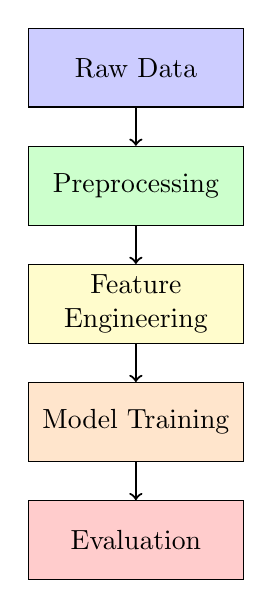
\begin{tikzpicture}[node distance=1.5cm, auto]
    \node (data) [rectangle, draw, fill=blue!20, text width=2.5cm, text centered, minimum height=1cm] {Raw Data};
    \node (preprocess) [rectangle, draw, fill=green!20, text width=2.5cm, text centered, minimum height=1cm, below of=data] {Preprocessing};
    \node (feature) [rectangle, draw, fill=yellow!20, text width=2.5cm, text centered, minimum height=1cm, below of=preprocess] {Feature Engineering};
    \node (model) [rectangle, draw, fill=orange!20, text width=2.5cm, text centered, minimum height=1cm, below of=feature] {Model Training};
    \node (evaluate) [rectangle, draw, fill=red!20, text width=2.5cm, text centered, minimum height=1cm, below of=model] {Evaluation};
    
    \draw[->, thick] (data) -- (preprocess);
    \draw[->, thick] (preprocess) -- (feature);
    \draw[->, thick] (feature) -- (model);
    \draw[->, thick] (model) -- (evaluate);
\end{tikzpicture}
\end{center}
\end{frame}

\begin{frame}{Preprocessing Techniques}
\begin{columns}[T]
\column{0.5\textwidth}
\textbf{Data Cleaning:}
\begin{itemize}
    \item Missing value imputation
    \begin{itemize}
        \item Median for numerical
        \item Mode for categorical
    \end{itemize}
    \item Duplicate removal
    \item Outlier detection
\end{itemize}

\column{0.5\textwidth}
\textbf{Feature Transformation:}
\begin{itemize}
    \item Label Encoding for categorical features
    \item StandardScaler normalization
    \item Feature scaling
    \item Optional PCA for dimensionality reduction
\end{itemize}
\end{columns}
\end{frame}

\begin{frame}{Machine Learning Models}
\begin{block}{Seven Classification Algorithms Evaluated}
\begin{enumerate}
    \item \textbf{Decision Tree} - High interpretability
    \item \textbf{Random Forest} - Ensemble method
    \item \textbf{LightGBM} - Gradient boosting framework
    \item \textbf{Naive Bayes} - Probabilistic classifier
    \item \textbf{Logistic Regression} - Linear baseline
    \item \textbf{AdaBoost} - Adaptive boosting
    \item \textbf{SGD Classifier} - Stochastic optimization
\end{enumerate}
\end{block}
\end{frame}

\begin{frame}{Feature Engineering}
\textbf{Strategies Implemented:}
\begin{itemize}
    \item \textbf{Interaction Terms}: Capture feature combinations
    \item \textbf{Polynomial Features}: Non-linear relationships
    \item \textbf{Domain-Specific Features}:
    \begin{itemize}
        \item Process information
        \item Network activity patterns
        \item File system characteristics
    \end{itemize}
    \item \textbf{Feature Selection}: Remove redundant features
\end{itemize}

\vspace{0.3cm}
\begin{alertblock}{Key Insight}
System properties like process info and network activity were most indicative of malware presence
\end{alertblock}
\end{frame}

% Section 4: Results
\section{Results}

\begin{frame}{Model Performance Comparison}
\begin{table}
\centering
\small
\begin{tabular}{@{}llccc@{}}
\toprule
\textbf{Model} & \textbf{Algorithm} & \textbf{Accuracy} & \textbf{Precision} & \textbf{Recall} \\
\midrule
Model 1 & Decision Tree & 85.20\% & 84.50\% & 86.10\% \\
Model 2 & Random Forest & 88.45\% & 87.80\% & 89.20\% \\
\textbf{Model 3} & \textbf{LightGBM} & \textbf{91.30\%} & \textbf{90.50\%} & \textbf{92.10\%} \\
Model 4 & Naive Bayes & 79.60\% & 78.90\% & 80.30\% \\
Model 5 & Logistic Reg. & 83.70\% & 83.20\% & 84.50\% \\
Model 6 & AdaBoost & 86.90\% & 86.30\% & 87.60\% \\
Model 7 & SGD Classifier & 82.40\% & 81.80\% & 83.20\% \\
\bottomrule
\end{tabular}
\end{table}

\vspace{0.2cm}
\begin{block}{Best Performer}
\textbf{LightGBM} achieved the highest accuracy at \textbf{91.30\%}
\end{block}
\end{frame}

\begin{frame}{Key Findings}
\begin{itemize}
    \item \textbf{LightGBM Performance}: Superior accuracy with efficient training
    \item \textbf{Ensemble Methods}: Random Forest and AdaBoost showed strong performance
    \item \textbf{Hyperparameter Tuning}: Improved performance by 2-5\% across models
    \item \textbf{Cross-Validation}: Consistent performance across folds indicates good generalization
    \item \textbf{Feature Importance}: Network activity and process information most significant
\end{itemize}
\end{frame}

\begin{frame}{Performance Insights}
\begin{columns}[T]
\column{0.5\textwidth}
\textbf{Strengths:}
\begin{itemize}
    \item High accuracy on test data
    \item Good balance between precision and recall
    \item Robust to overfitting
    \item Efficient training time
\end{itemize}

\column{0.5\textwidth}
\textbf{Advantages:}
\begin{itemize}
    \item Modular architecture
    \item Production-ready code
    \item Comprehensive evaluation
    \item Interpretable results
\end{itemize}
\end{columns}
\end{frame}

% Section 5: Implementation
\section{Implementation}

\begin{frame}{System Architecture}
\textbf{Modular Pipeline Components:}
\begin{enumerate}
    \item \textbf{Data Loading}: CSV file handling with pandas
    \item \textbf{Preprocessing Module}: Configurable data cleaning
    \item \textbf{Feature Engineering}: Optional transformation steps
    \item \textbf{Model Training}: Multiple algorithm support
    \item \textbf{Evaluation}: Comprehensive metrics and visualization
    \item \textbf{Prediction}: Automated submission generation
\end{enumerate}

\vspace{0.3cm}
\textbf{Technology Stack:}
\begin{itemize}
    \item Python 3.11, scikit-learn, LightGBM
    \item pandas, numpy, matplotlib
\end{itemize}
\end{frame}

\begin{frame}{Code Organization}
\begin{block}{Configuration-Driven Design}
Selective enabling/disabling of:
\begin{itemize}
    \item Preprocessing steps
    \item Feature engineering techniques
    \item Model selection
    \item Hyperparameter tuning
\end{itemize}
\end{block}

\vspace{0.3cm}

\textbf{Benefits:}
\begin{itemize}
    \item Easy experimentation
    \item Maintainable codebase
    \item Model persistence and logging
    \item Reproducible results
\end{itemize}
\end{frame}

% Section 6: Conclusion
\section{Conclusion}

\begin{frame}{Key Contributions}
\begin{enumerate}
    \item \textbf{Comprehensive Model Comparison}: Systematic evaluation of seven algorithms
    
    \item \textbf{Modular Pipeline}: Flexible, configuration-driven architecture
    
    \item \textbf{Robust Preprocessing}: Complete data handling pipeline
    
    \item \textbf{Automated Optimization}: Hyperparameter tuning integration
    
    \item \textbf{Production-Ready}: Maintainable codebase with model persistence
    
    \item \textbf{Superior Performance}: 91.30\% accuracy with LightGBM
\end{enumerate}
\end{frame}

\begin{frame}{Practical Implications}
\begin{itemize}
    \item \textbf{Early Threat Detection}: Proactive malware identification
    \item \textbf{Scalability}: Efficient algorithms for large-scale deployment
    \item \textbf{Interpretability}: Feature importance for analyst understanding
    \item \textbf{Flexibility}: Multiple models for different requirements
    \item \textbf{Cost-Effectiveness}: Automated detection reduces manual effort
\end{itemize}
\end{frame}

\begin{frame}{Future Work}
\begin{columns}[T]
\column{0.5\textwidth}
\textbf{Technical Enhancements:}
\begin{itemize}
    \item Deep learning integration
    \item Real-time deployment
    \item Ensemble methods
    \item Explainable AI (SHAP, LIME)
    \item Active learning
\end{itemize}

\column{0.5\textwidth}
\textbf{Practical Extensions:}
\begin{itemize}
    \item Multi-class classification
    \item SIEM integration
    \item Adversarial robustness
    \item Transfer learning
    \item Automated feature engineering
\end{itemize}
\end{columns}
\end{frame}

\begin{frame}{Limitations}
\begin{alertblock}{Current Limitations}
\begin{itemize}
    \item Depends on training data quality and representativeness
    \item Performance may degrade with new malware variants
    \item Manual feature engineering process
    \item Requires periodic retraining
    \item Real-time optimization needs investigation
\end{itemize}
\end{alertblock}
\end{frame}

\begin{frame}{Resources}
\begin{block}{Project Resources}
\textbf{Kaggle Competition:}\\
\url{https://www.kaggle.com/competitions/System-Threat-Forecaster/}

\vspace{0.3cm}

\textbf{Implementation Notebook:}\\
\url{https://www.kaggle.com/code/milavdabgar/system-threat-forecaster-modular}
\end{block}

\vspace{0.3cm}

\textbf{Technologies:} Python 3.11, scikit-learn, LightGBM, pandas, numpy, matplotlib
\end{frame}

% Thank You Slide
\begin{frame}
\begin{center}
{\Huge Thank You!}

\vspace{1cm}

{\Large Questions?}

\vspace{1cm}

\textbf{Milav Jayeshkumar Dabgar}\\
Government Polytechnic Palanpur\\
Department of Electronics and Communication Engineering

\end{center}
\end{frame}

\end{document}
